\documentclass[letterpaper, 10 pt, conference]{ieeeconf}
\IEEEoverridecommandlockouts
\overrideIEEEmargins

\usepackage{graphicx}
\usepackage{amsmath}
\usepackage{amssymb}
\usepackage{cite}
\usepackage{url}
\usepackage{balance}

\title{\LARGE \bf
Three Ways to Use VLMs in Robot Learning:\\
Real2Sim, Failure Detection, and Inference-Time Steering
}

\author{Kaneyoshi Hiratsuka}

\begin{document}

\maketitle
\thispagestyle{empty}
\pagestyle{empty}

\begin{abstract}
Vision--language models (VLMs) such as GPT-6 Astra show a step change in spatial reasoning, and agentic frameworks such as ASPIRE~\cite{lu2026aspire} that let a model write robot skills as code reach 99\% success on the 80-task LIBERO-Pro suite. A VLM used directly as a policy, however, is still weak at precise, contact-rich and bimanual manipulation. This resume surveys three recent papers that instead use the VLM \emph{around} a pretrained policy. SimFoundry~\cite{ranawaka2026simfoundry} (Real2Sim) turns one video into a physics-ready simulation scene and its variants, giving sim evaluations that predict real performance ($r=0.911$) and sim-to-real training data. Code-as-Monitor~\cite{zhou2025codeasmonitor} (failure detection) has a VLM write monitor code over geometric constraint elements, unifying reactive and proactive detection in real time. VLS~\cite{liu2026vls} (steering) has a VLM write differentiable rewards whose gradients steer the denoising of a frozen diffusion or flow-matching policy. We summarize each work and discuss their common pattern: VLM-written geometry and code used to build simulators, monitor execution, and steer generation.
\end{abstract}

\section{INTRODUCTION}

Foundation models are starting to solve manipulation benchmarks. GPT-6 Astra (OpenAI, Sep.~2026) is widely used to write code that drives robots directly, and ASPIRE~\cite{lu2026aspire}, an agentic skill-discovery framework from NVIDIA GEAR, lets a coding agent write, test and revise robot skills as programs; its v1.0 reaches 99\% on LIBERO-Pro, and success rises with the strength of the base model (15\% with GPT-6 Luna, 99\% with Claude Opus 5.5). Yet a VLM used directly as the policy reports only 22.5\% on RoboDojo: semantic reasoning outruns physical execution. A natural alternative is to keep a pretrained policy, such as a vision--language--action (VLA) model or a diffusion policy, as the motor-skill prior and to use the VLM's spatial understanding, reasoning and code generation around it. We organize this idea into three areas and review one paper for each: \emph{Real2Sim} (SimFoundry), \emph{failure detection} (Code-as-Monitor) and \emph{inference-time steering} (VLS).

\section{PAPER 1: SIMFOUNDRY (REAL2SIM)}

\begin{figure}[t]
  \centering
  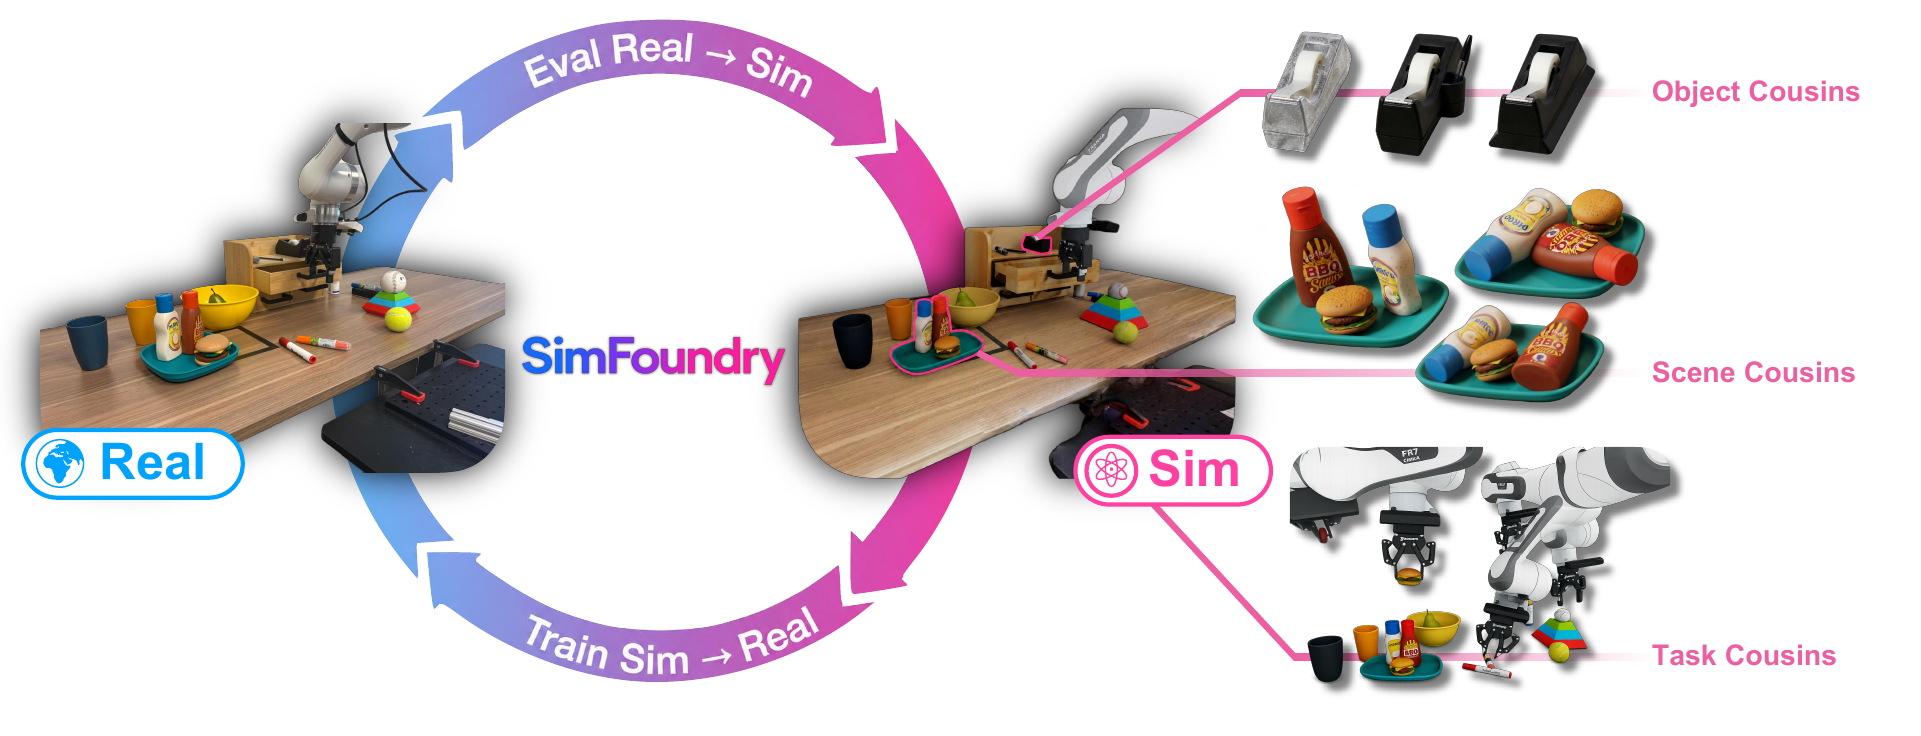
\includegraphics[width=0.72\columnwidth]{figs/sf_fig1.png}
  \caption{SimFoundry builds a digital twin from one video and expands it into object, scene and task cousins for real-to-sim evaluation and sim-to-real training. Reproduced from~\cite{ranawaka2026simfoundry}.}
  \label{fig:sf}
\end{figure}

\textbf{Background.} Training robot foundation models needs months of teleoperation and evaluating them needs thousands of real trials. Simulation scales, and sim evaluations have been shown to correlate with real results, but building sim scenes that match the real world by hand is the bottleneck. No existing real-to-sim system covers training, evaluation and automatic construction together with systematic diversification.

\textbf{Method.} SimFoundry~\cite{ranawaka2026simfoundry} is a modular three-stage pipeline (Fig.~\ref{fig:sf}). \emph{Extraction} picks a frame, estimates depth, detects objects with a VLM and segments them one at a time with SAM~3, inpainting each away. \emph{Generation} turns each crop into a textured mesh with a 2D-to-3D model, aligns its pose with FoundationPose, infers joints for articulated objects, builds collision geometry with CoACD, assigns mass and friction via a VLM, stabilizes the scene in PyBullet and exports it to simulators such as IsaacLab; every module is replaceable. \emph{Augmentation} expands the twin into digital cousins: object cousins perturb an object image and regenerate the mesh, scene cousins let a VLM edit spatial predicates such as \texttt{OnTop}, and task cousins let a VLM propose new tasks that are converted to BDDL goals and demonstrated automatically.

\textbf{Results.} Seven tasks on a DROID Franka and a bimanual YAM with five policies ($\pi_0$, $\pi_{0.5}$, GR00T N1.6/N1.7, DreamZero) give a mean Pearson correlation of 0.911 and MMRV of 0.018 between sim and real success, more than 0.59 above PolaRiS in correlation and without fine-tuning the policies to sim; sub-task evaluation raises $r$ to 0.95. Policies trained only on sim data reach 99\% (Pot on Stove, YAM) and 100\% (Stack Dishware, DROID) zero-shot on the real robots, and object, scene and task cousins add 17, 21 and 40 points on average. Reconstruction reaches zero-shot F1 of 0.81--0.92 at about five minutes per object; the main limitation is the tabletop assumption.

\section{PAPER 2: CODE-AS-MONITOR (FAILURE DETECTION)}

\begin{figure}[t]
  \centering
  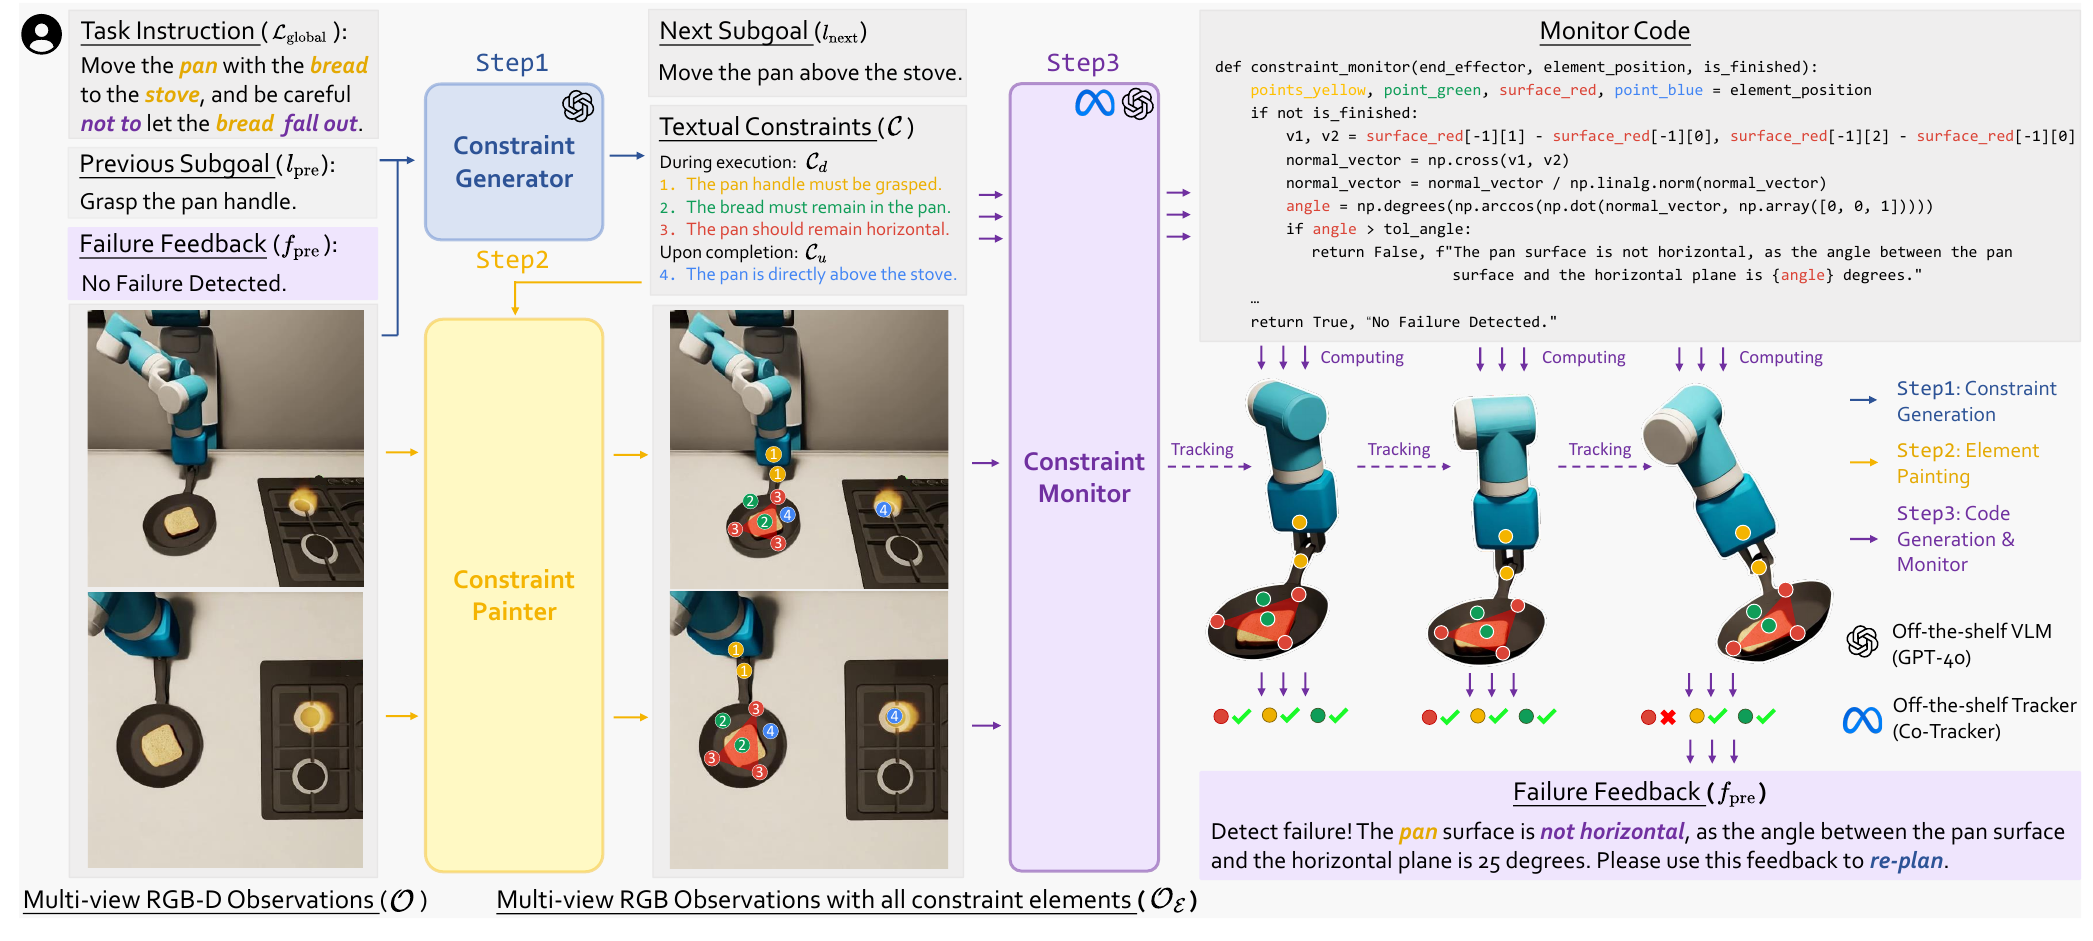
\includegraphics[width=0.8\columnwidth]{figs/cam_fig2.png}
  \caption{Code-as-Monitor. A VLM writes constraints, the Painter maps them to constraint elements, and VLM-generated code monitors the tracked elements in real time. Reproduced from~\cite{zhou2025codeasmonitor}.}
  \label{fig:cam}
\end{figure}

\textbf{Background.} \emph{Reactive} detection identifies a failure after it occurs; \emph{proactive} detection prevents a foreseeable one. Prior work asks a VLM about failures as visual question answering, which is slow and coarse in 3D, and proactive open-set detection was largely unexplored.

\textbf{Method.} Code-as-Monitor (CaM)~\cite{zhou2025codeasmonitor} formulates both modes as spatio-temporal constraint satisfaction (Fig.~\ref{fig:cam}). GPT-4o generates the next subgoal with constraints to maintain during execution (proactive, e.g., ``the pan should remain horizontal'') and upon completion (reactive, e.g., ``the pan is above the stove''). The relevant parts are abstracted into \emph{constraint elements}, points, lines and surfaces, by ConSeg, a LISA-based segmentation model trained with LoRA on 10,181 BridgeData~V2 trajectories auto-annotated by GPT-4o; masks are lifted to 3D, clustered and connected, then annotated on multi-view images. Prompted with these images, GPT-4o writes monitor code that takes element positions and their history, computes angles and distances, and returns a failure flag with a reason. The VLM is called once per subgoal; afterwards elements are tracked with CoTracker and the code runs every frame. On a violation the policy halts and the reason triggers re-planning.

\textbf{Results.} In CLIPort under severe disturbances CaM reaches 88.3\% versus 76.7\% for DoReMi, and counting element points raises ``sweep half the blocks'' from 16.7\% to 75.0\%. In OmniGibson only CaM detects surface-level disturbances, while cutting execution time by 34.8\% and tokens by 52.2\%; on RLBench it improves ARP from 91.3\% to 97.1\% on unseen articulated and tool-use tasks. On a real UR5 with a Leap Hand and the open-loop grasp model DexGraspNet~2.0, CaM exceeds 90\% under disturbances and reaches 90\% on a cluttered reasoning task where DoReMi scores 0\%. Ablations show that multi-view input, constraint-aware segmentation and point connection each matter.

\section{PAPER 3: VLS (INFERENCE-TIME STEERING)}

\begin{figure}[t]
  \centering
  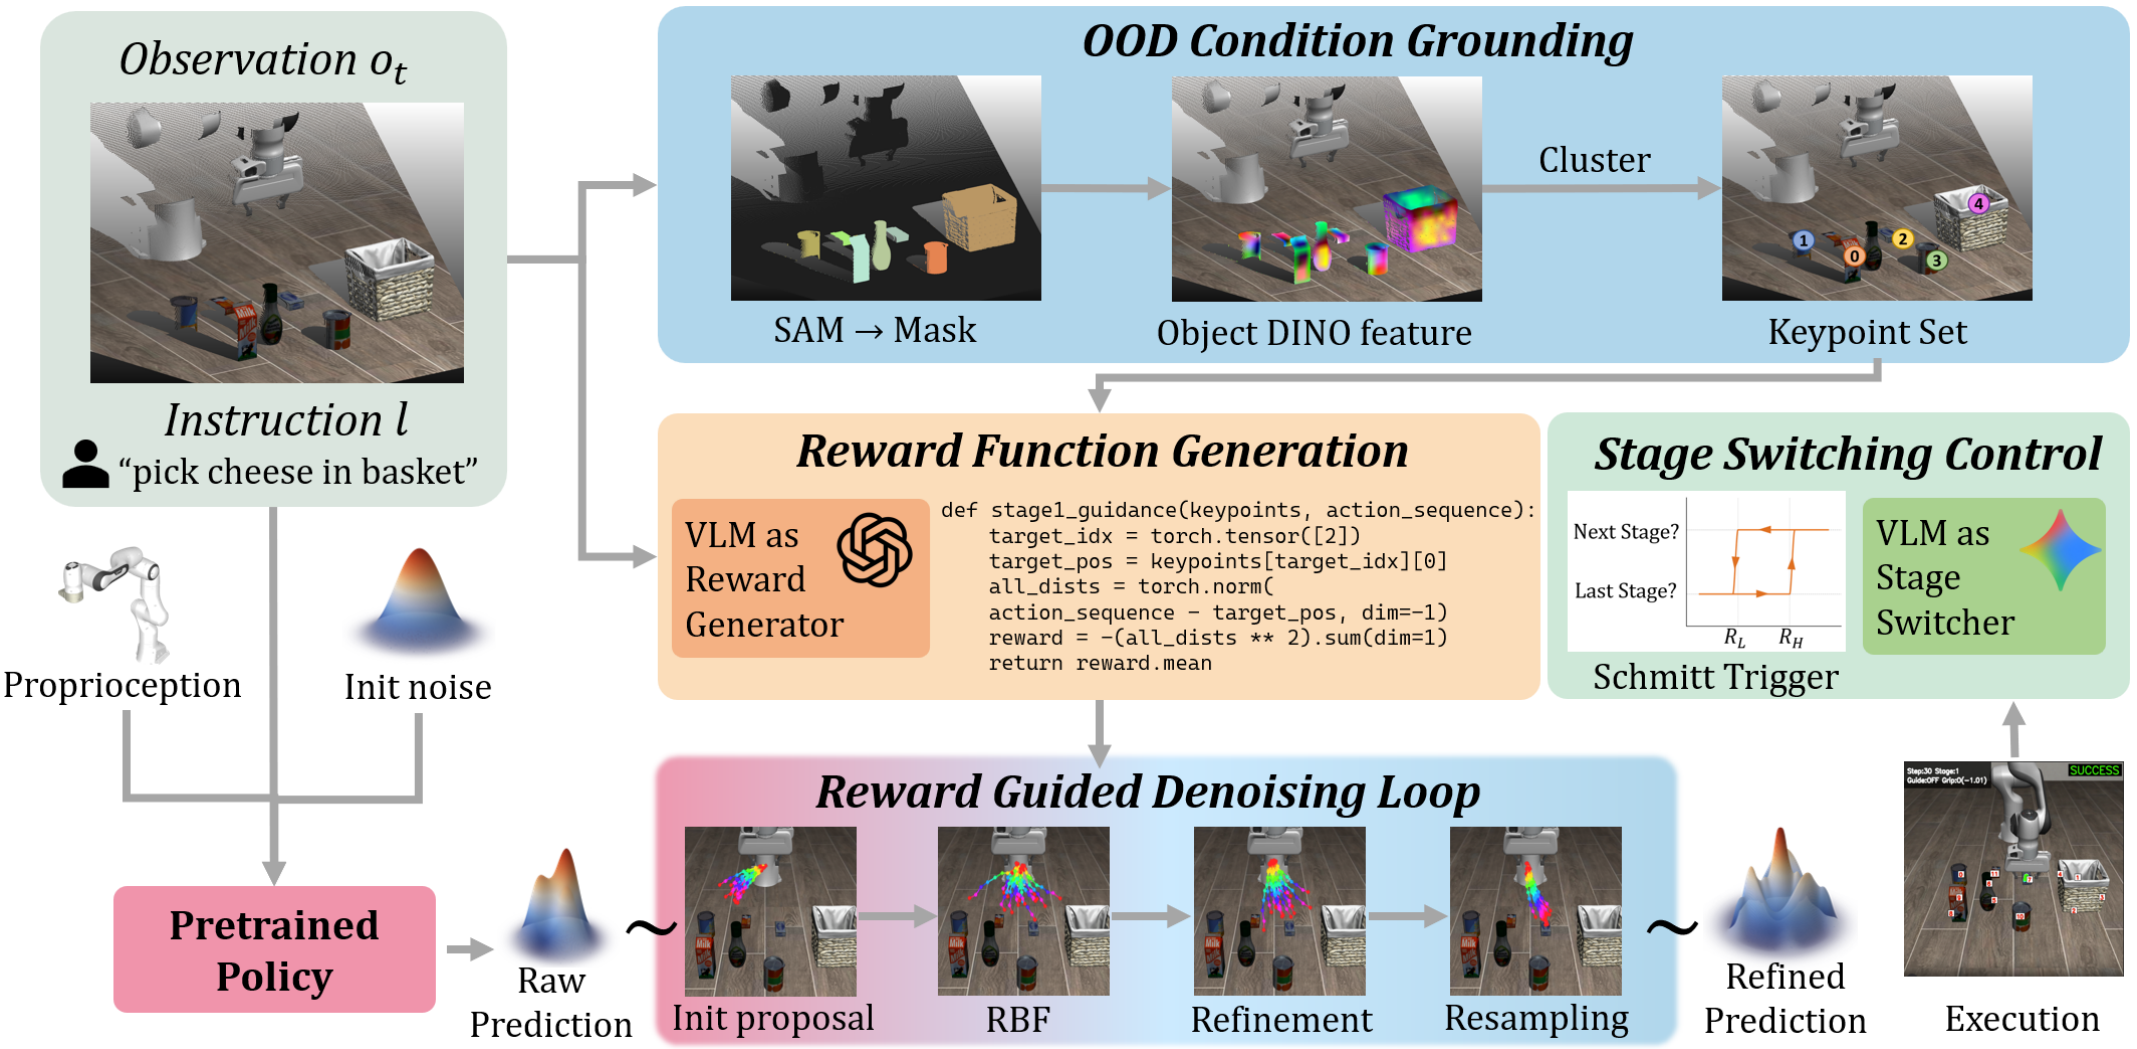
\includegraphics[width=0.8\columnwidth]{figs/vls_fig2.png}
  \caption{VLS. The input is grounded into 3D keypoints, a VLM writes stage-wise differentiable rewards, and their gradients steer the denoising loop of a frozen policy with RBF diversity and Feynman--Kac resampling. Reproduced from~\cite{liu2026vls}.}
  \label{fig:vls}
\end{figure}

\textbf{Background.} Diffusion and flow-matching policies fail under mild shifts such as a nearby obstacle or a moved support surface. VLS~\cite{liu2026vls} argues the skills exist but are coupled to training-time layouts and instructions, so adaptation should be treated as inference-time control rather than retraining.

\textbf{Method.} VLS steers a frozen policy $\pi^\star$ with classifier guidance, $\hat v = v(a^k,(o,l)_{\mathrm{OOD}},k)+\lambda g$ with $g\approx\nabla_{a^k}R(a^k;\mathcal{P})$ (Fig.~\ref{fig:vls}). (i) \emph{Grounding}: SAM, DINOv2 and depth turn the observation into task-relevant 3D keypoints $\mathcal{P}$. (ii) \emph{Reward generation}: a VLM splits the task into stages and writes each stage's reward over $\mathcal{P}$ and the action sequence as differentiable PyTorch code, staying outside the computation graph itself. (iii) \emph{Guided denoising}: a batch of candidates is kept diverse by RBF repulsion, refined by repeated reward-gradient steps, and resampled with Feynman--Kac weights $G_i^k=\exp R_s(a^k[i])$. The guidance strength $\lambda$ adapts to the reward relative to the first chunk of a stage, and a Schmitt-trigger hysteresis switches stages, querying the VLM for the next reward.

\textbf{Results.} On LIBERO-PRO, adding VLS to a frozen LeRobot $\pi_{0.5}$ raises success from 23.7\% to 36.8\%, while OpenVLA and $\pi_0$ stay near 0\%. On CALVIN with a diffusion-policy base, VLS reaches 94\% on movable objects (7.4$\times$) and 87\% on articulated parts (9.6$\times$), 15--25 points above DynaGuide and ITPS; removing gradient guidance collapses success to 17\%. On a real Franka with frozen $\pi_{0.5}$, in-distribution success rises from 50\% to 69\% and out-of-distribution from 42\% to 69\%, including 40\% on an unseen mug where the baseline fails. The main limitation is latency of about one second per action chunk.

\section{DISCUSSION AND CONCLUSIONS}
All three papers use the VLM around a pretrained policy rather than as the policy. SimFoundry exploits VLM spatial understanding to copy real scenes into simulation and generate diverse data; Code-as-Monitor and VLS both have the VLM write geometric elements and code over them, differing only in whether the code is a monitor condition that checks execution or a reward that steers generation. As ASPIRE shows, methods in which the model writes code improve with the base model. Their shared costs are latency and VLM errors. A promising direction, which the author is exploring on LIBERO, is to combine steering and monitoring so that the same VLM-written code guides generation and checks execution, and to accumulate sim-verified code as a reusable asset so that real-robot deployment depends less on inference-time VLM calls.

\balance
\bibliographystyle{ieeetr}
\bibliography{../references}

\end{document}
